\chapter{Laboratorio 5}
Il primo circuito realizzato in questa esperienza di laboratorio permette di effettuare lo switch debouncing attraverso l'integrato LM555. Nella figura \ref{fig:circuito_1} è riportato lo schema del circuito.
\begin{figure}[h!]
	\centering
	\begin{minipage}{.45\textwidth}
		\scalebox{.47}{
			\begin{circuitikz}
				%Main dip package
				\draw (0,0) node[dipchip,num pins=8, hide numbers, external pins width=0.1, scale=3, external pad fraction=6](C){LM555};
				%Pin names
				\node [right] at (C.bpin 1) {GND};
				\node [right] at (C.bpin 2) {Trigger};
				\node [right] at (C.bpin 3) {Output};
				\node [right] at (C.bpin 4) {Reset};
				\node [left] at (C.bpin 5) {Control Voltage};
				\node [left] at (C.bpin 6) {Threshold};
				\node [left] at (C.bpin 7) {Discharge};
				\node [left] at (C.bpin 8) {$V_{CC}$};
				%Connections
				\draw (C.pin 1) -- ++(-2.9,0) ++(-.1,0) node[jump crossing](crgnd){} ++(-.1,0) -- ++(-.9,0) -- ++(0,-6) node[ground]{};
				\draw (C.pin 8) -- ++(2,0) coordinate(vcc) -- ++(0,1.35) node[vcc]{$V_{CC}$};
				\draw (C.pin 7) -- ++(2,0) coordinate(dsc) to[R=$R$] (vcc);
				\draw (C.pin 6) -- ++(2,0) coordinate(trs) -- (dsc);
				\draw (trs) -- ++(2,0) to[C=$C$] ++(0,-2.68) node[ground]{};
				\draw (C.pin 5) -- ++(2,0) to[C=$C_2$] ++(0,-1) node[ground]{};
				\draw (C.pin 4) -- ++(-1.5,0) -- ++(0,3) to[crossing] ++(0,.72) to[crossing] ++ (0,2.64) node[vcc]{$V_{CC}$};
				\draw (C.pin 3) to[short, -o] ++(-1,0) ++(0,.1) node[above]{$v_{out}$};
				\draw (C.pin 2) -- ++(-3,0) coordinate(vin);
				\draw (vin) to[nopb=$SW_{T}$] ++(0,-4.32) node[ground]{};
				\draw (vin) to[R=$R_2$] (crgnd) -- ++(0,1.33) node[vcc]{$V_{CC}$};
				\draw[thick] (-7.5,-5.3) rectangle (8,5.9);
			\end{circuitikz}
		}
	\end{minipage}\qquad
	\begin{minipage}{.45\textwidth}
		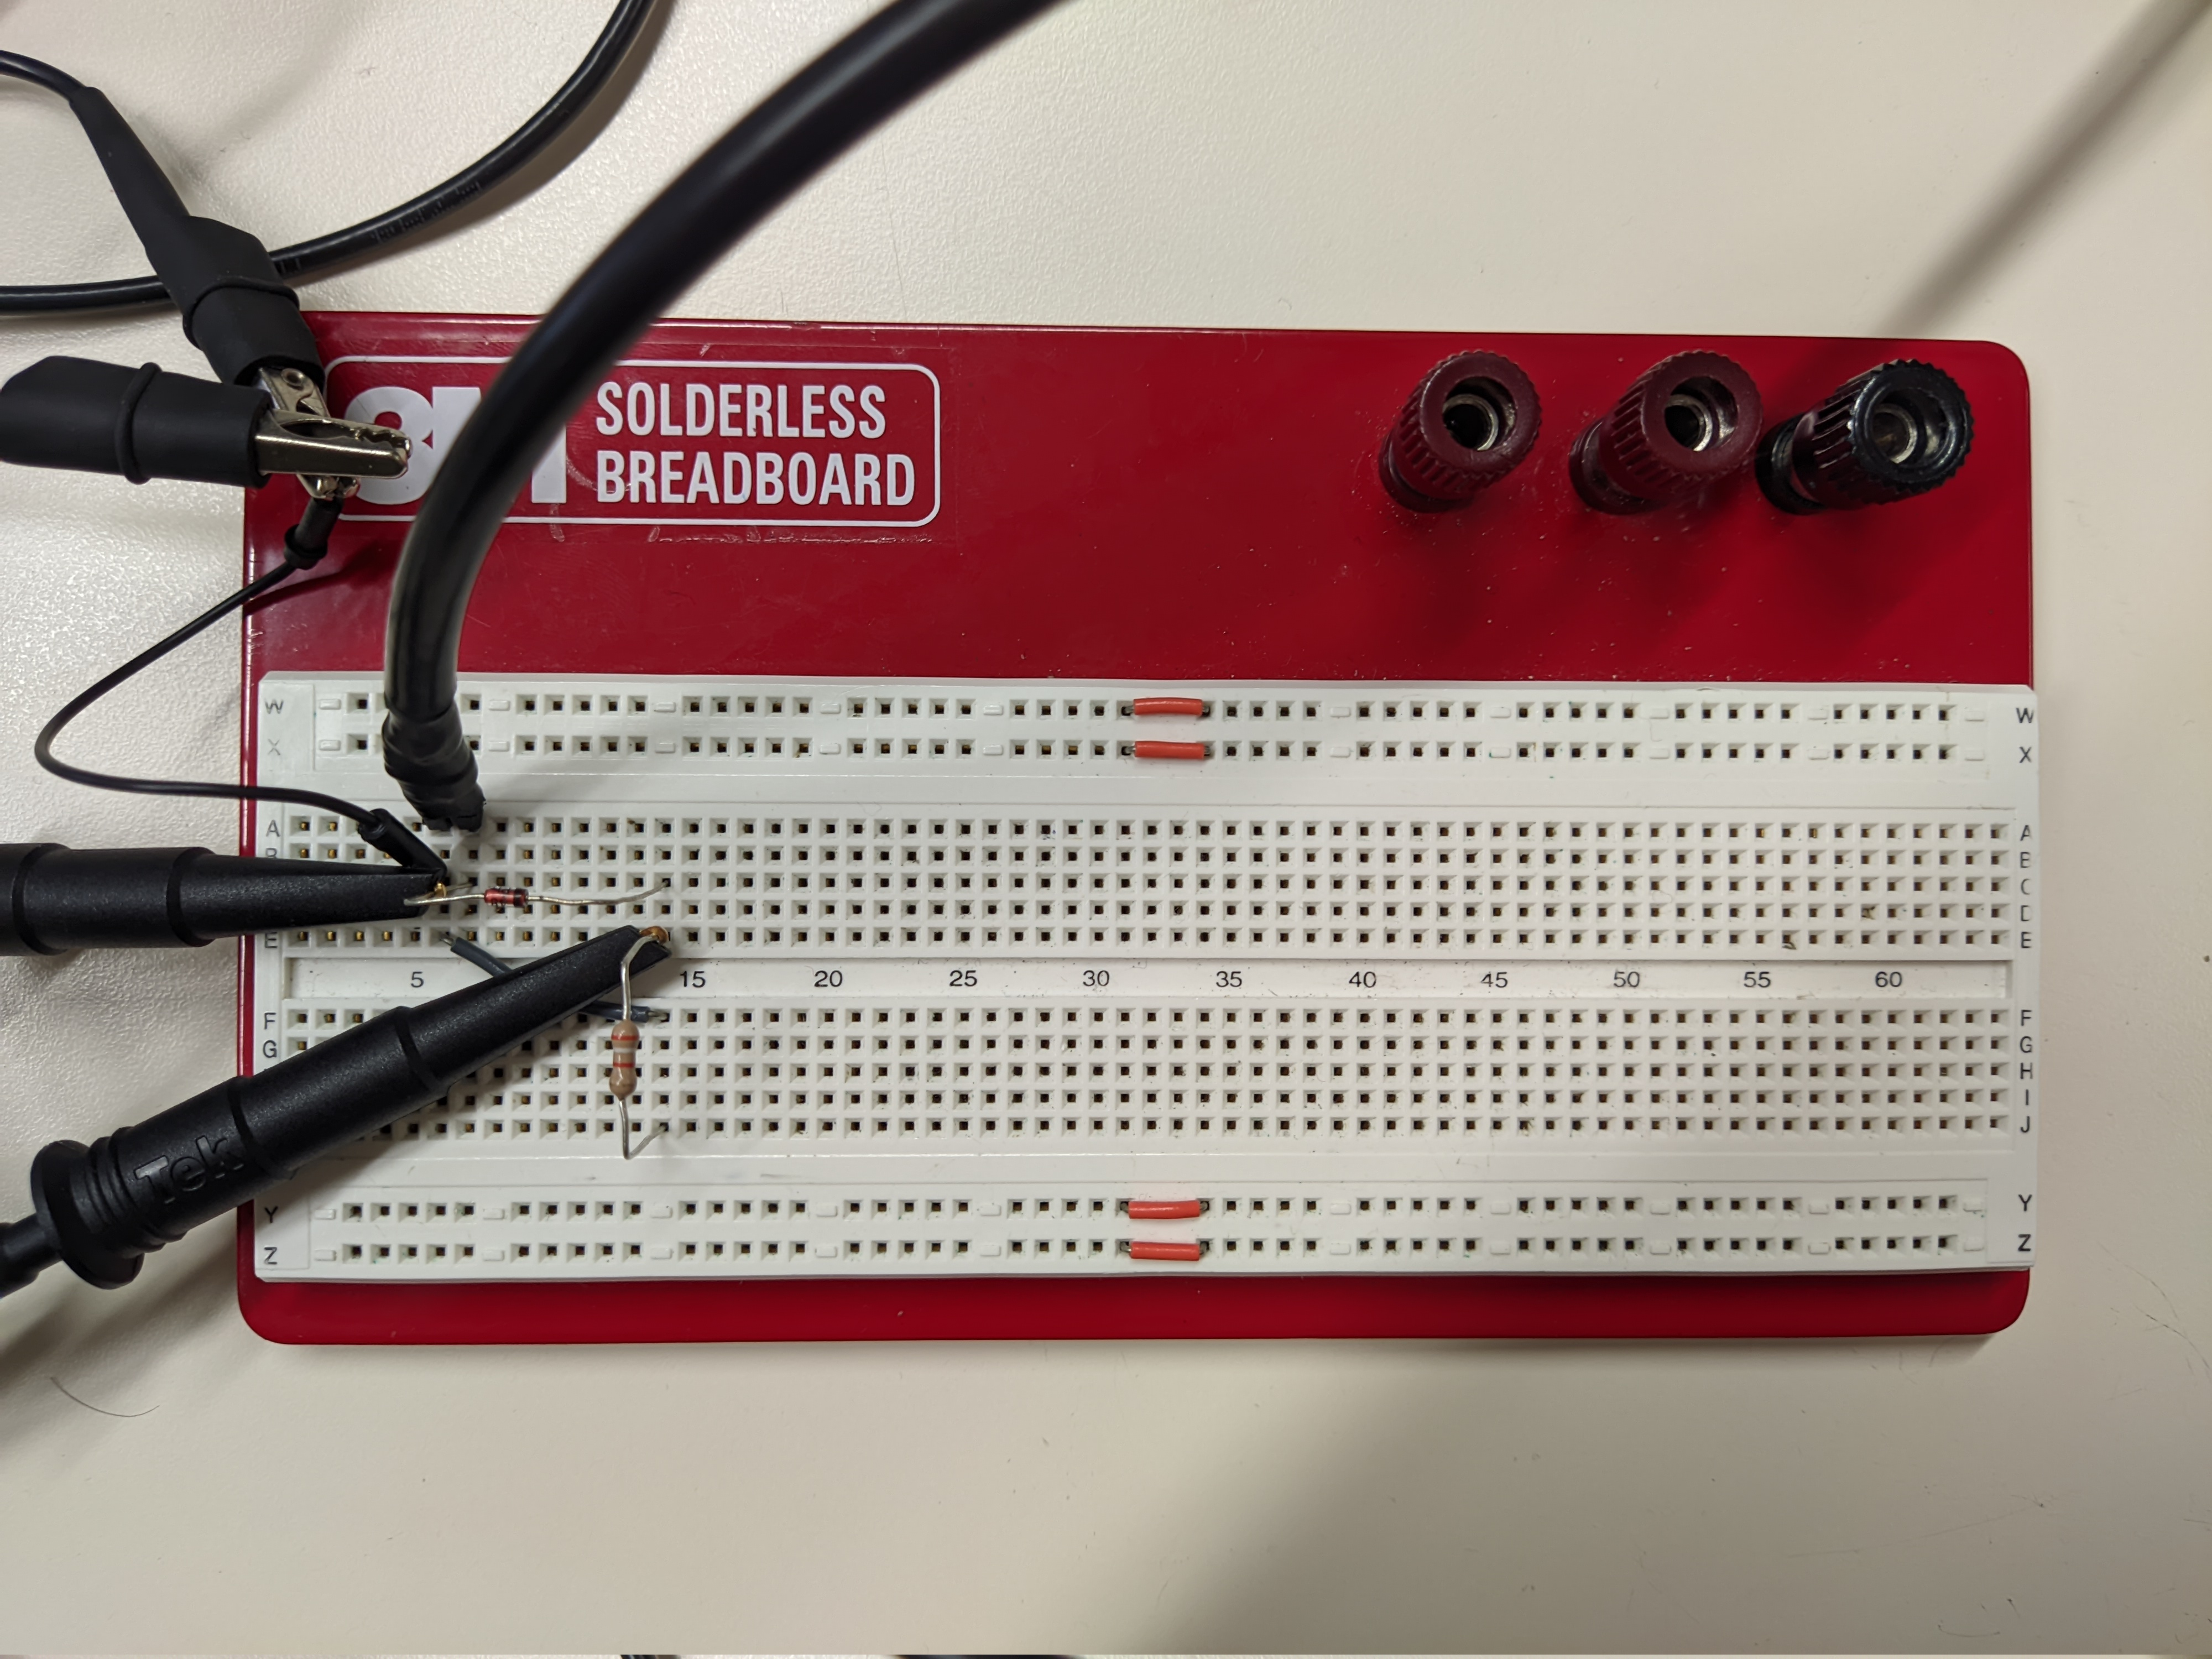
\includegraphics[width=\linewidth]{./ImageFiles/Laboratorio 5/CIR1.jpg}
	\end{minipage}
	\caption{Schema circuitale e foto del circuito realizzato.}
	\label{fig:circuito_1}
\end{figure}

\noindent
In questo circuito il Timer 555 è utilizzato in configurazione monostabile. A differenza del circuito realizzato nella relazione precedente, il segnale di trigger viene generato non più tramite il generatore di forme d'onda ma tramite un pulsante meccanico normalmente aperto, indicato nello schema circuitale con il nome di $SW_{T}$. 
Esso ha un terminale connesso alla resistenza $R_2$ di pull-up verso $V_{CC}$, mentre l'altro terminale è connesso a massa. Per cui, quando l'interruttore è aperto sul nodo di \textit{Trigger} viene mantenuta una tensione di $V_{CC}$ grazie alla resistenza $R_2$. Quando l'interruttore viene chiuso invece il morsetto di \textit{Trigger} viene collegato a massa. Tuttavia, la risposta reale di un pulsante meccanico durante l'apertura e la chiusura è influenzata dalla propria risposta meccanica, caratterizzata dal fenomeno del rimbalzo (\textit{switch bouncing}). A causa di questo effetto, si possono notare degli impulsi di apertura-chiusura quando viene premuto o rilasciato il pulsante (\Fig\ref{fig:switch_bouncing}).
\begin{figure}[tbh]
	\centering
	\begin{minipage}{.496\textwidth}
		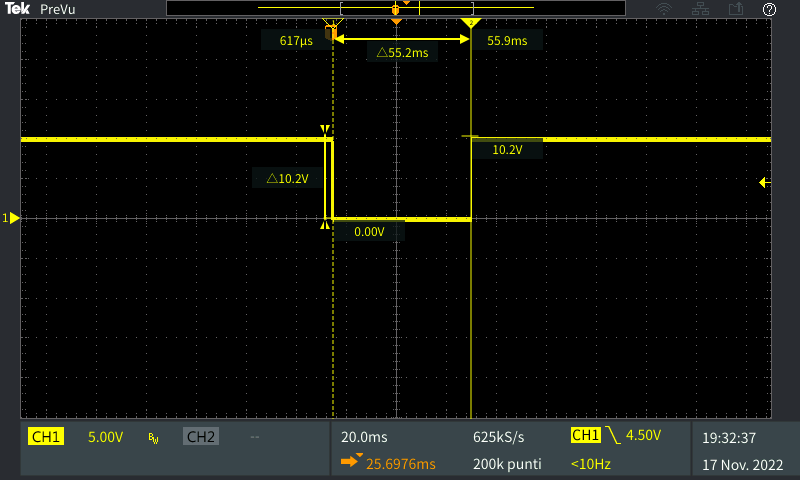
\includegraphics[width=\linewidth]{./ImageFiles/Laboratorio 5/TEK00003.PNG}
	\end{minipage}
	\begin{minipage}{.496\textwidth}
		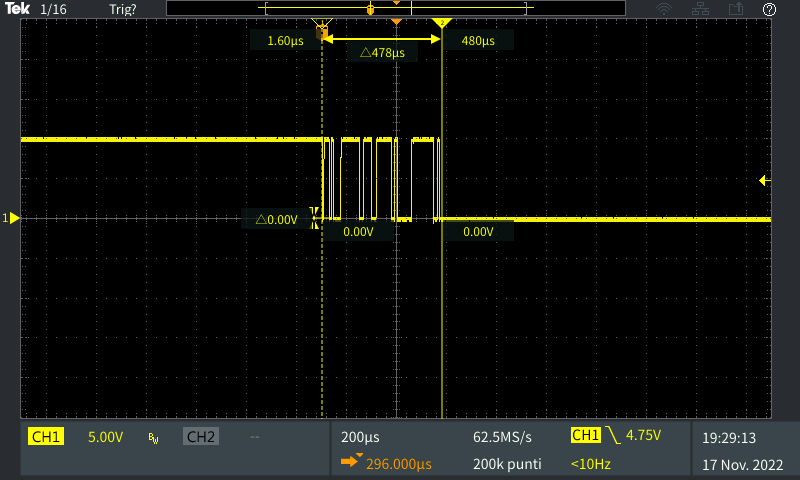
\includegraphics[width=\linewidth]{./ImageFiles/Laboratorio 5/TEK00002.PNG}
	\end{minipage}
	\caption{Effetto rimbalzo durante l'apertura e la chiusura di un pulsante meccanico. A sinistra è possibile vedere il segnale ai morsetti del pulsante quando viene premuto per circa \SI{55.2}{\milli\second}. A destra un dettaglio sul segnale alla pressione del pulsante in cui l'effetto del rimbalzo dura circa \SI{478}{\micro\second}.}
	\label{fig:switch_bouncing}
\end{figure}
Questo comportamento anomalo potrebbe presentare un problema quando è inserito, per esempio, in un circuito digitale che conta quante volte è stato premuto il pulsante: il circuito contatore conterà anche le oscillazioni causate dal rimbalzo. Per superare questo problema è possibile sfruttare il \textbf{LM555} in modalità monostabile che, a seguito di un impulso negativo sul trigger genera un impulso in uscita con durata pari a $T=1.1RC$. Il circuito quindi realizzato può essere utilizzato per ottenere un singolo impulso in uscita a seguito della pressione del pulsante collegato al morsetto di trigger. Nella figura \ref{fig:circuito_1_scope} viene confrontato l'andamento della tensione al morsetto di trigger e la tensione in uscita al timer 555. I valori dei componenti passivi utilizzati per questa misura sono indicati nella tabella \ref{tab:valori_componenti_1}.

\def\arraystretch{1.3}
\begin{table}[h!]
	\centering
	\begin{tabular}{|c|c|c|}
		\hline
		Componente	& Valore Nominale & Valore Misurato \\ \hline
		$R_2$ &\SI{12}{\kilo\ohm} & \SI{10.96}{\kilo\ohm} \\ \hline
		$R$ &\SI{270}{\kilo\ohm} & \SI{265.8}{\kilo\ohm} \\ \hline
		$C$ &\SI{330}{\nano\farad} & Non misurato \\ \hline
	\end{tabular}
	\caption{Valori nominali e misurati dei componenti utilizzati nel circuito.}
	\label{tab:valori_componenti_1}
\end{table}
\begin{figure}[tbh]
	\centering
	\begin{minipage}{.496\textwidth}
		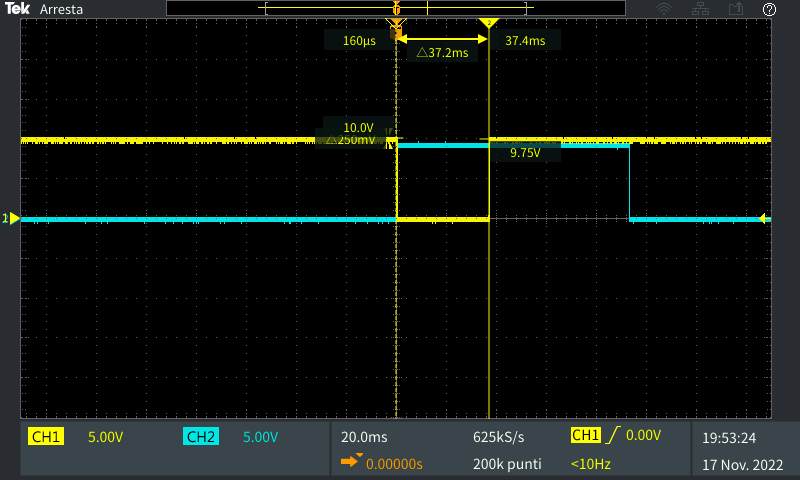
\includegraphics[width=\linewidth]{./ImageFiles/Laboratorio 5/TEK00005.PNG}
	\end{minipage}
	\begin{minipage}{.496\textwidth}
		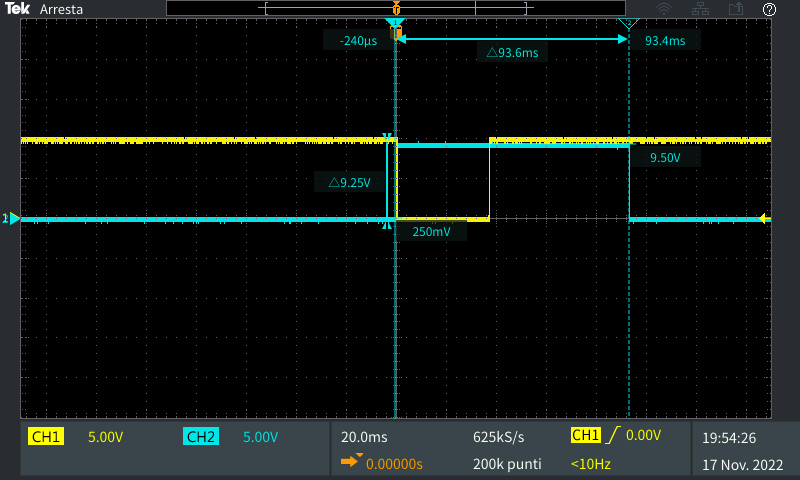
\includegraphics[width=\linewidth]{./ImageFiles/Laboratorio 5/TEK00006.PNG}
	\end{minipage}
	\caption{Uscita al LM555 (linea azzurra) in configurazione monostabile e tensione al morsetto di trigger (linea gialla).}
	\label{fig:circuito_1_scope}
\end{figure}



\clearpage
Il secondo circuito realizzato utilizza \textbf{LM555} in modalità bistabile (\Fig\ref{fig:circuito_2}) e permette di generare un impulso rettangolare in uscita al time 555 di durata controllabile dalla pressione di due pulsanti: un pulsante di trigger ($SW_T$) e uno di reset ($SW_R$).
\begin{figure}[h!]
	\centering
	\begin{minipage}{.45\textwidth}
		\scalebox{.47}{
			\begin{circuitikz}
				%Main dip package
				\draw (0,0) node[dipchip,num pins=8, hide numbers, external pins width=0.1, scale=3, external pad fraction=6](C){LM555};
				%Pin names
				\node [right] at (C.bpin 1) {GND};
				\node [right] at (C.bpin 2) {Trigger};
				\node [right] at (C.bpin 3) {Output};
				\node [right] at (C.bpin 4) {Reset};
				\node [left] at (C.bpin 5) {Control Voltage};
				\node [left] at (C.bpin 6) {Threshold};
				\node [left] at (C.bpin 7) {Discharge};
				\node [left] at (C.bpin 8) {$V_{CC}$};
				%Connections
				\draw (C.pin 1) -- ++(-2.9,0) ++(-.1,0) node[jump crossing](crgnd){} ++(-.1,0) -- ++(-.9,0) -- ++(0,-6.5) node[ground]{};
				\draw (C.pin 8) -- ++(2,0) coordinate(vcc) -- ++(0,1.35) node[vcc]{$V_{CC}$};
				\draw (C.pin 7) -- ++(2,0) coordinate(dsc) to[R=$R$] (vcc);
				\draw (C.pin 6) -- ++(2,0) coordinate(trs) -- (dsc);
				\draw (trs) -- ++(2,0) to[C=$C$] ++(0,-3.18) node[ground]{};
				\draw (C.pin 5) -- ++(2,0) to[C=$C_2$] ++(0,-1.5) node[ground]{};
				\draw (C.pin 4) -- ++(-1.5,0) coordinate(swres) to[R=$R_3$] ++(0,1.5) -- ++(0,1.5) to[crossing] ++(0,.72) to[crossing] ++ (0,2.64) node[vcc]{$V_{CC}$};
				\draw (swres) to[nopb=$SW_{R}$] ++(0,-1.5) node[ground]{};
				\draw (C.pin 3) to[short, -o] ++(-1,0) ++(0,.1) node[above]{$v_{out}$};
				\draw (C.pin 2) -- ++(-3,0) coordinate(vin);
				\draw (vin) to[nopb=$SW_{T}$] ++(0,-2.82) -- +(0,-2) node[ground]{};
				\draw (vin) to[R=$R_2$] (crgnd) -- ++(0,1.33) node[vcc]{$V_{CC}$};
				\draw[thick] (-7.5,-5.3) rectangle (8,5.9);
			\end{circuitikz}
		}
	\end{minipage}\qquad
	\begin{minipage}{.45\textwidth}
		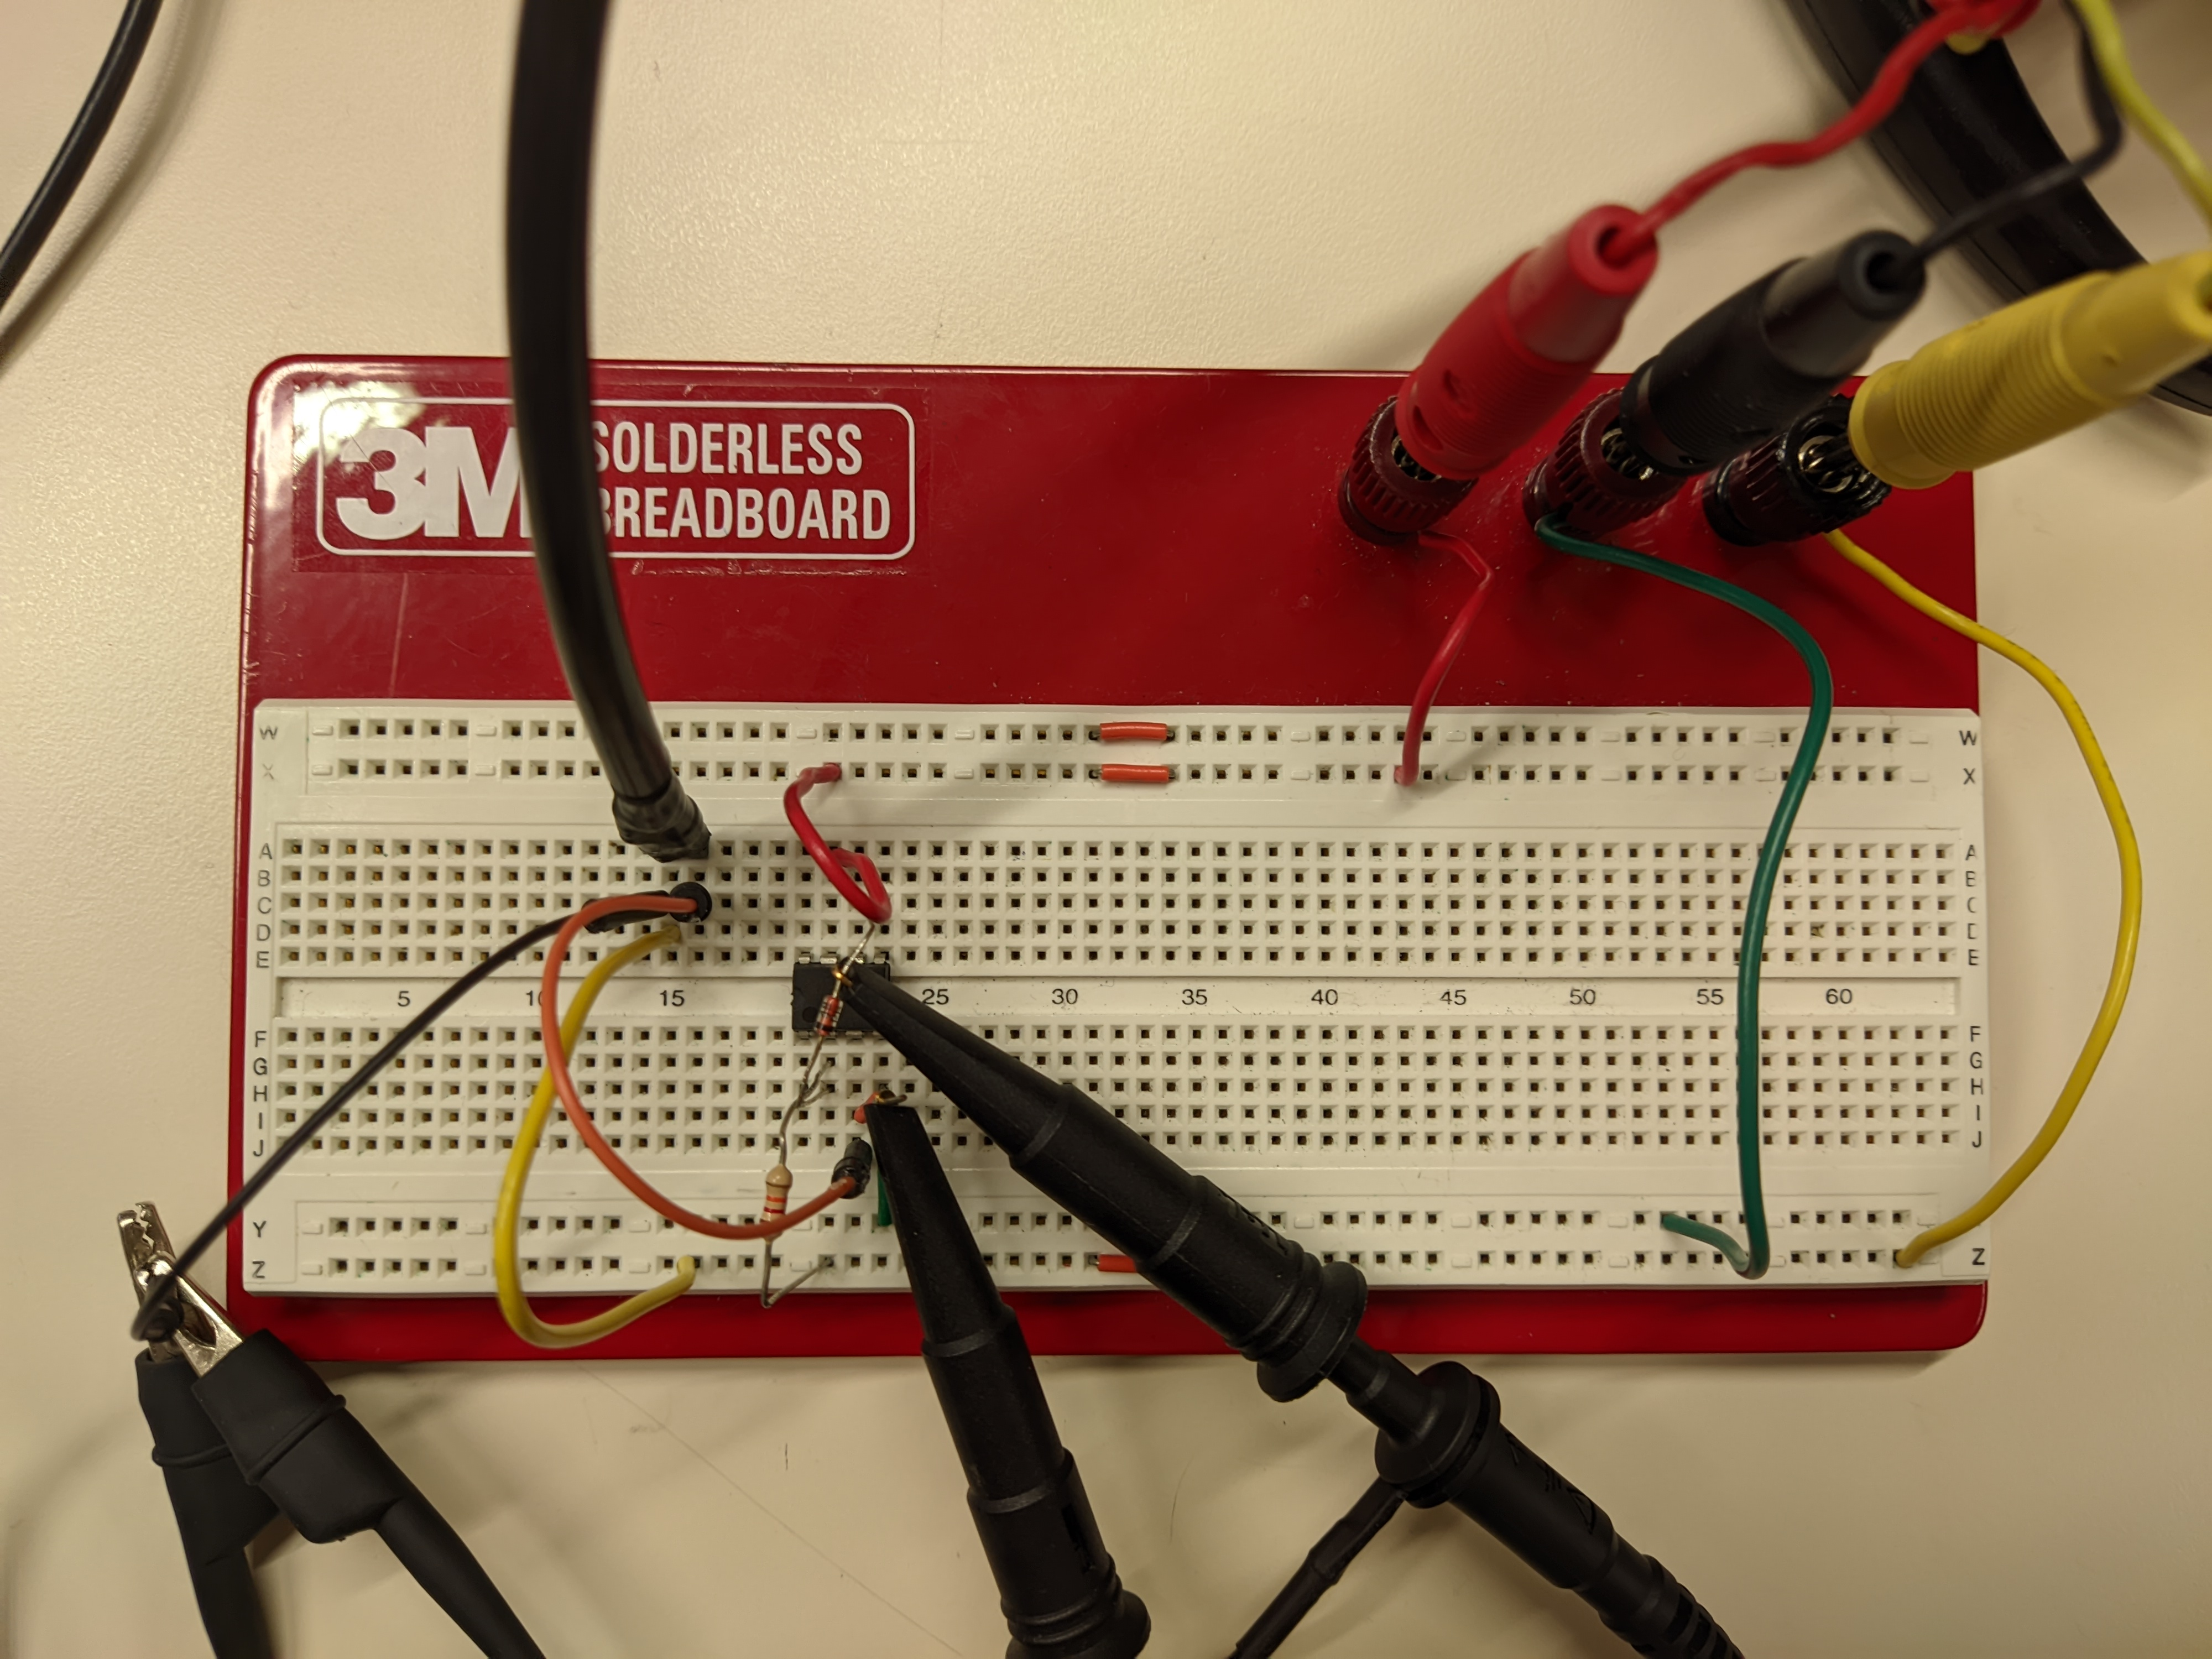
\includegraphics[width=\linewidth]{./ImageFiles/Laboratorio 5/CIR2.jpg}
	\end{minipage}
	\caption{Schema circuitale e foto del circuito realizzato.}
	\label{fig:circuito_2}
\end{figure}
\noindent
La configurazione astabile permette di ottenere in uscita un impulso rettangolare che viene generato a seguito di un impulso di trigger e termina quando sul morsetto di \textit{Reset} viene applicato un impulso. Infatti, il pin di \textit{Reset} è collegato internamente al pin di reset generale del \textit{flip-flop SR}, che porta l'uscita a zero qualsiasi siano i valori dei pin di set e reset. Il circuito quindi rimane stabile in uno dei due stati fino a quando il pulsante di reset o di trigger viene premuto. In realtà, nel circuito realizzato in laboratorio non si sono utilizzati due pulsati: il pulsante di reset è stato realizzato con un filo che viene collegato a massa e che simula la chiusura dell'interruttore. I valori dei componenti sono indicati nella tabella \ref{tab:valori_componenti_2}.
\def\arraystretch{1.3}
\begin{table}[h!]
	\centering
	\begin{tabular}{|c|c|c|}
		\hline
		Componente	& Valore Nominale & Valore Misurato \\ \hline
		R &\SI{270}{\kilo\ohm} & \SI{265,8}{\kilo\ohm} \\ \hline
		R2 &\SI{12}{\kilo\ohm} & \SI{10,96}{\kilo\ohm} \\ \hline
		R3 & \SI{12}{\kilo\ohm} & \SI{12}{\kilo\ohm} \\ \hline
		C & \SI{330}{\nano\farad} & Non misurato \\ \hline
		C2 & \SI{150}{\nano\farad} & Non misurato \\ \hline
	\end{tabular}
	\caption{Valori nominali e misurati dei componenti utilizzati nel circuito.}
	\label{tab:valori_componenti_2}
\end{table}
Nella figura \ref{fig:circuito_2_scope} viene rappresentata la fase di reset dell'uscita: dopo aver premuto il pulsante di trigger, l'uscita si porta a livello logico alto pari a \SI{10}{\volt} (linea azzurra). Successivamente, quando il pulsante di reset $SW_R$ viene premuto (o collegando il pin di reset a massa) viene generato un impulso negativo sul pin di reset (linea gialla). Dopo un tempo di ritardo pari a \SI{43}{\milli\second} l'uscita si riporta a livello logico basso (\SI{0}{\volt}).
\begin{figure}[tbh]
	\centering
	\begin{minipage}{.496\textwidth}
		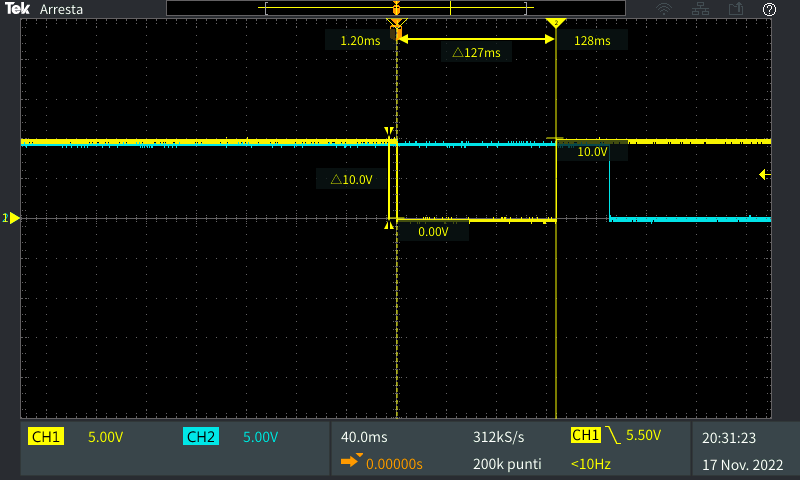
\includegraphics[width=\linewidth]{./ImageFiles/Laboratorio 5/TEK00010.PNG}
	\end{minipage}
	\begin{minipage}{.496\textwidth}
		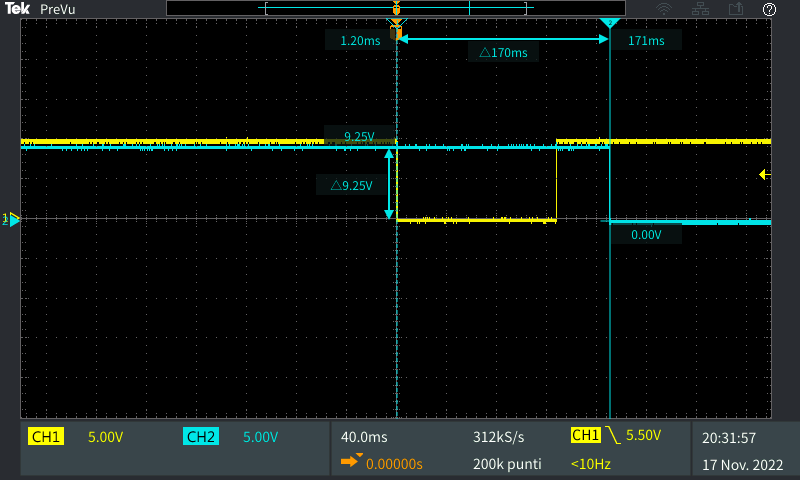
\includegraphics[width=\linewidth]{./ImageFiles/Laboratorio 5/TEK00011.PNG}
	\end{minipage}
	\caption{Reset del segnale in uscita al LM555 (linea azzurra) in configurazione bistabile a seguito di un impulso (linea gialla) sul pin di reset.}
	\label{fig:circuito_2_scope}
\end{figure}

\clearpage
Il terzo circuito realizzato utilizza il timer 555 per realizzare un oscillatore che permette di generare in uscita un'onda quadra periodica con un periodo definito dai valori dei componenti passivi utilizzati nel circuito, indicati nella tabella \ref{tab:valori_componenti_3}.
\begin{figure}[h!]
	\centering
	\begin{minipage}{.45\textwidth}
		\scalebox{.47}{
			\begin{circuitikz}
				%Main dip package
				\draw (0,0) node[dipchip,num pins=8, hide numbers, external pins width=0.1, scale=3, external pad fraction=6](C){LM555};
				%Pin names
				\node [right] at (C.bpin 1) {GND};
				\node [right] at (C.bpin 2) {Trigger};
				\node [right] at (C.bpin 3) {Output};
				\node [right] at (C.bpin 4) {Reset};
				\node [left] at (C.bpin 5) {Control Voltage};
				\node [left] at (C.bpin 6) {Threshold};
				\node [left] at (C.bpin 7) {Discharge};
				\node [left] at (C.bpin 8) {$V_{CC}$};
				%Connections
				\draw (C.pin 1) -- ++(-2.9,0) ++(-.1,0) node[jump crossing](crgnd){} ++(-.1,0) -- ++(-.9,0) -- ++(0,-6.5) node[ground]{};
				\draw (C.pin 8) -- ++(.9,0) ++(.1,0) coordinate(vccj) node[jump crossing]{} ++(.1,0)-- ++(.9,0) coordinate(vcc) -- ++(0,1.35) node[vcc]{$V_{CC}$};
				\draw (C.pin 7) -- ++(2,0) coordinate(dsc) to[R=$R_A$] (vcc);
				\draw (C.pin 5) -- ++(.9,0) ++(.1,0) node[jump crossing]{} ++(.1,0) -- ++(.9,0) to[C=$C_2$] ++(0,-1.5) node[ground]{};
				\draw (C.pin 6) -- ++(1,0) -- ++(0,-3.6) -- ++(-8.9,0) to[short, -*] ++(0,5.28);
				\draw (C.pin 4) -- ++(-1.5,0) -- ++(0,3) to[crossing] ++(0,.72) to[crossing] ++ (0,2.64) node[vcc]{$V_{CC}$};
				\draw (C.pin 3) to[short, -o] ++(-1,0) ++(0,.1) node[above]{$v_{out}$};
				\draw (C.pin 2) -- ++(-3,0) coordinate(vin);
				\draw (vin) to[R=$R_B$] (crgnd) -- ++(0,2.5) coordinate(tb) -- (tb-|vccj) -- (vccj) to[short, -*] (C.pin 7 -| vccj);
				\draw (vin) to[C=$C$] ++(0,-4.82) node[ground]{};
				\draw[thick] (-8,-5.3) rectangle (6.6,5.9);
			\end{circuitikz}
		}
	\end{minipage}\qquad
	\begin{minipage}{.45\textwidth}
		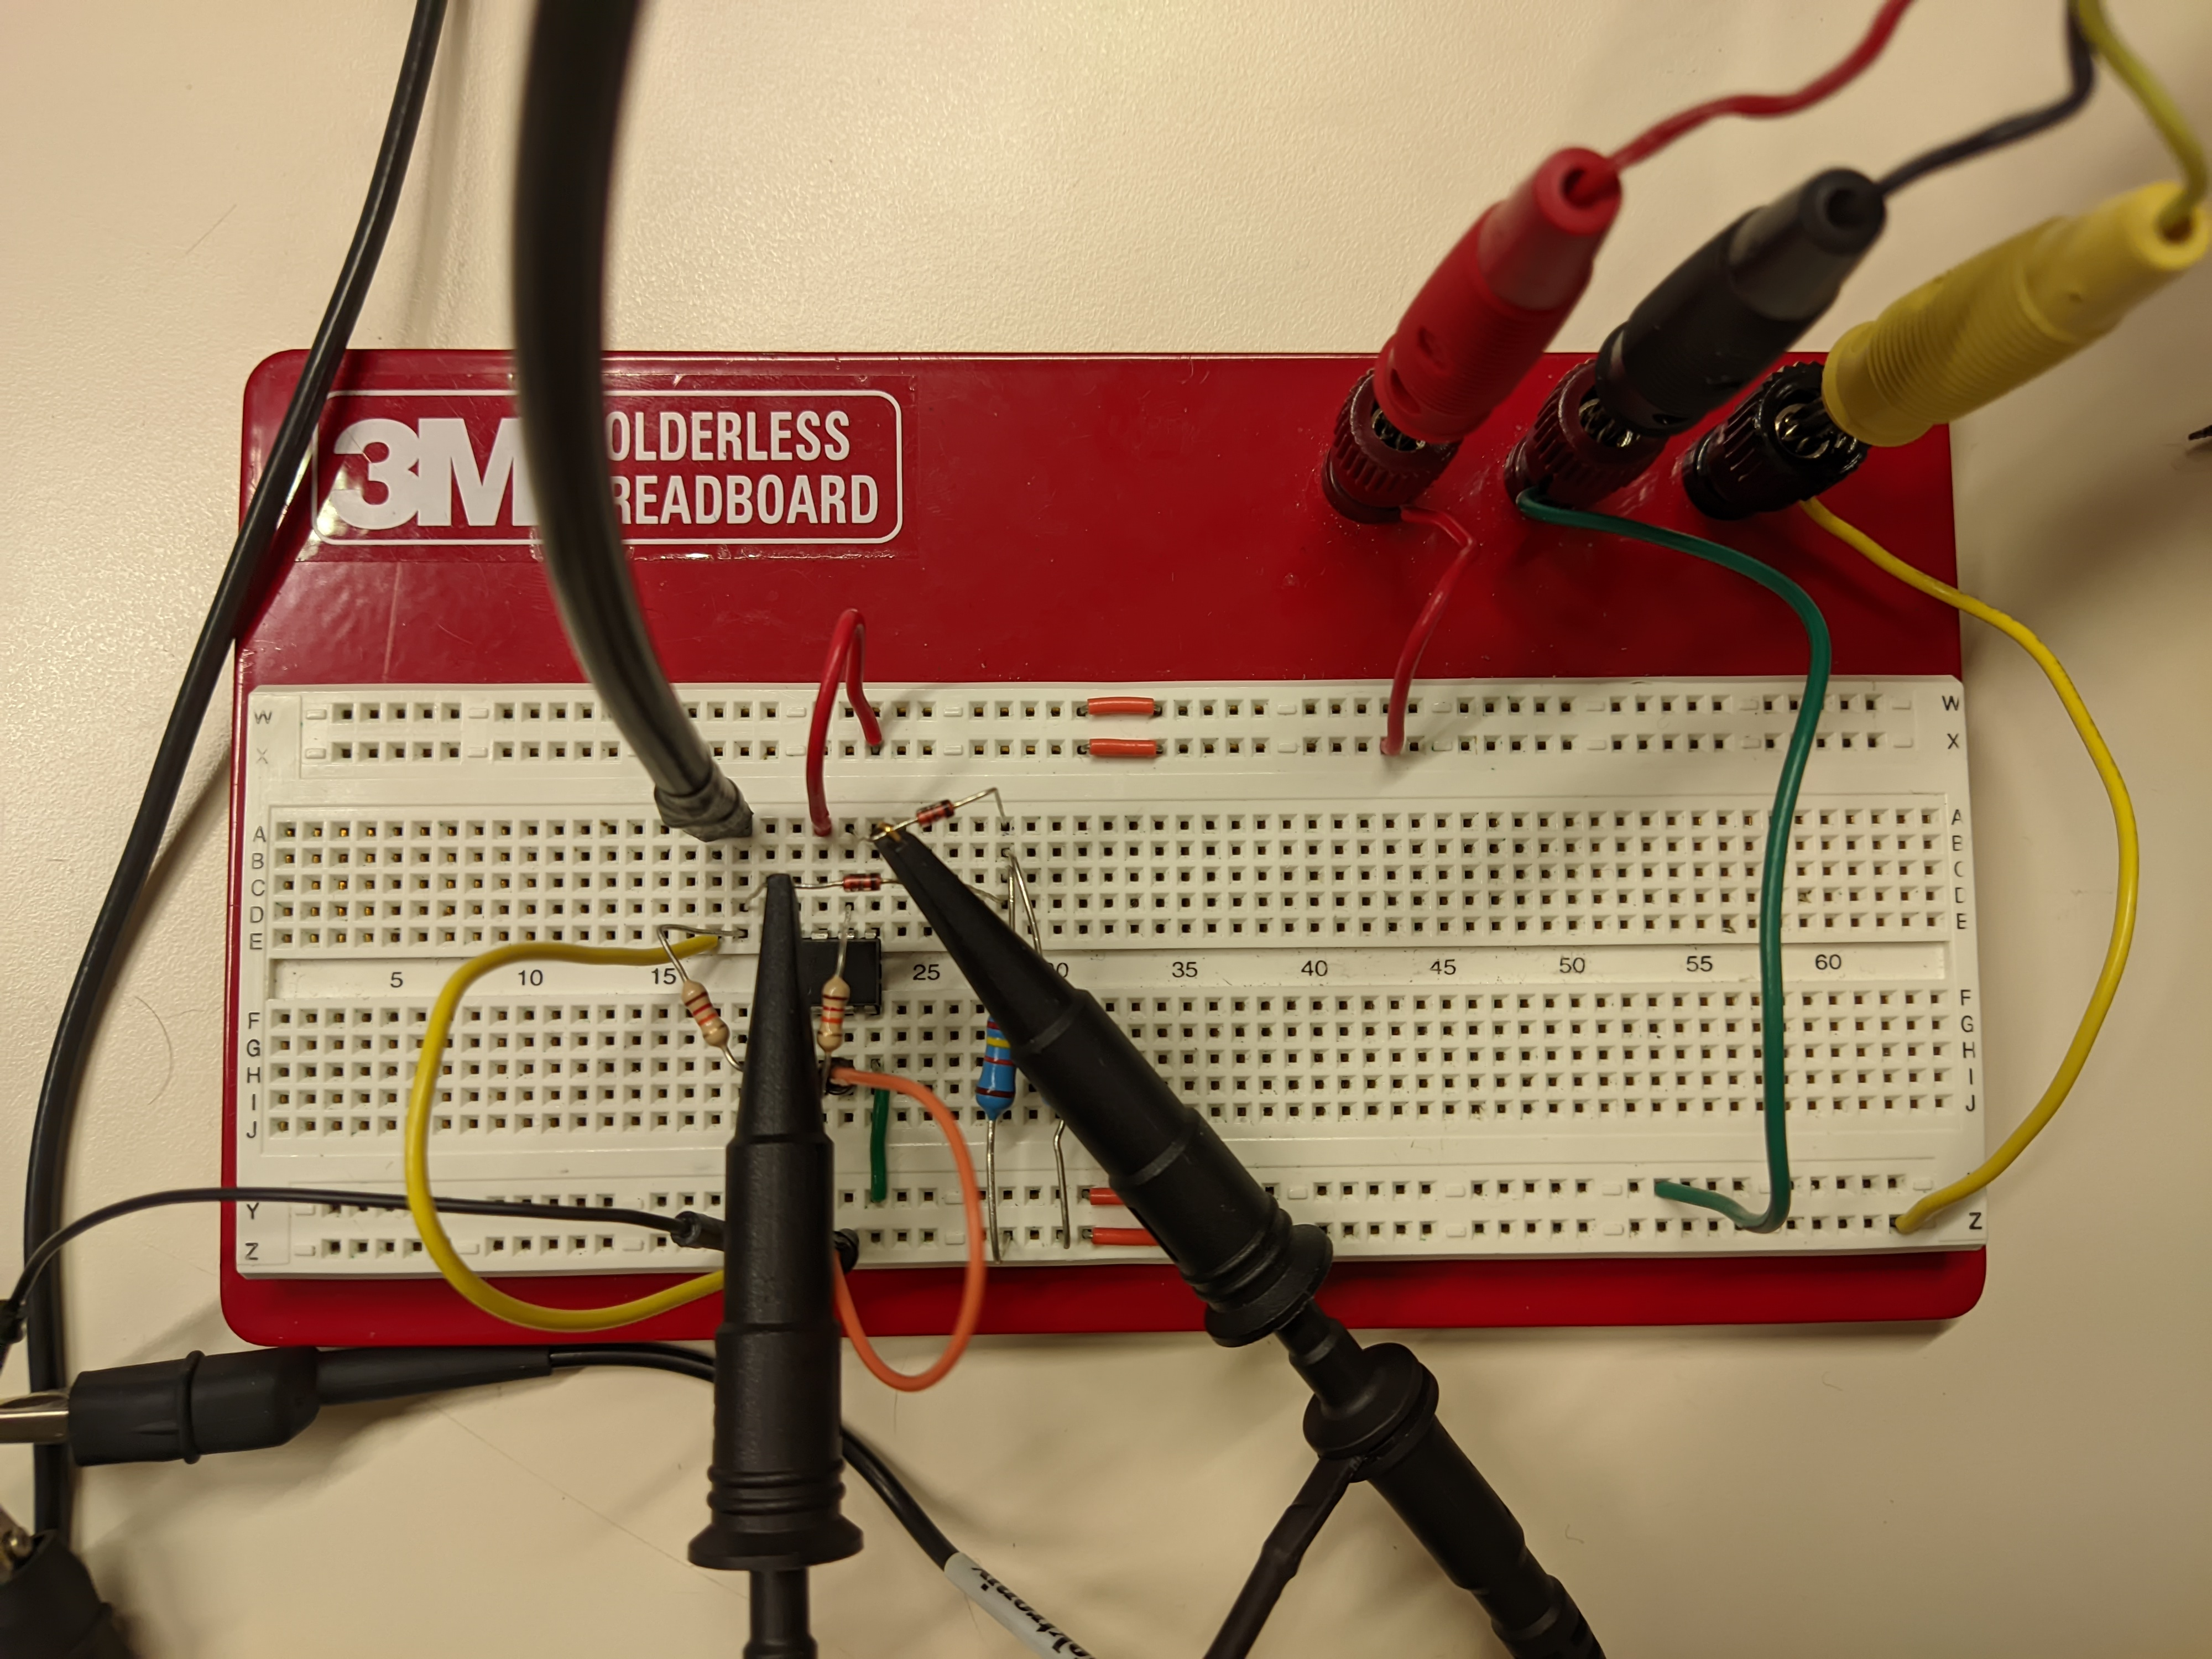
\includegraphics[width=\linewidth]{./ImageFiles/Laboratorio 5/CIR3.jpg}
	\end{minipage}
	\caption{Schema circuitale e foto del circuito realizzato.}
	\label{fig:circuito_3}
\end{figure}

\def\arraystretch{1.3}
\begin{table}[h!]
	\centering
	\begin{tabular}{|c|c|c|}
		\hline
		Componente	& Valore Nominale & Valore Misurato \\ \hline
		$R_{A_{12k}}$ &\SI{12}{\kilo\ohm} & \SI{10.96}{\kilo\ohm} \\ \hline
		$R_{A_{18k}}$ &\SI{18}{\kilo\ohm} & \SI{18.02}{\kilo\ohm} \\ \hline
		$R_{A_{23k}}$ &\SI{23}{\kilo\ohm} & \SI{23.90}{\kilo\ohm} \\ \hline
		$R_{A_{39k}}$ &\SI{39}{\kilo\ohm} & \SI{38.65}{\kilo\ohm} \\ \hline
		$R_{A_{50k}}$ &\SI{50}{\kilo\ohm} & \SI{55.10}{\kilo\ohm} \\ \hline
		$R_{A_{66k}}$ &\SI{66}{\kilo\ohm} & \SI{66.87}{\kilo\ohm} \\ \hline
		$R_{A_{82k}}$ &\SI{82}{\kilo\ohm} & \SI{82.26}{\kilo\ohm} \\ \hline
		$R_B$ &\SI{12}{\kilo\ohm} & \SI{12.00}{\kilo\ohm} \\ \hline
		$C$ & \SI{330}{\nano\farad} & Non misurato \\ \hline
		$C_2$ & \SI{150}{\nano\farad} & Non misurato \\ \hline
	\end{tabular}
	\caption{Valori nominali e misurati dei componenti utilizzati nel circuito.}
	\label{tab:valori_componenti_3}
\end{table}
In questa configurazione, il condensatore $C$ inizia a caricarsi attraverso le resistenze $R_A$ e $R_B$. Quando la tensione al nodo $v_c$ è pari a $\frac{2}{3}V_{CC}$ il \textit{flip-flop} viene resettato e quindi l'uscita del timer 555 va a livello logico basso e il transistor MOSFET di scarica si accende. La capacità si scarica quindi verso massa tramite la resistenza $R_B$ fino a quando la tensione al nodo $v_C$ si porta al valore $\frac{V_{CC}}{3}$. A questo punto, il \textit{flip-flop} viene settato e l'uscita si porta a livello logico alto, spegnendo il transistor di carica: il ciclo di carica inizia di nuovo. Il duty-cycle del segnale generato in uscita dipende dal tempo di carica e scarica della capacità $C$. Considerando il condensatore inizialmente carico a $\frac{V_{CC}}{3}$, l'andamento della tensione $v_C$ nella fase di carica è pari a:
\begin{equation}
	\begin{split}
		v_C&=V_{CC}+\left(\frac{V_{CC}}{3}-V_{CC}\right)e^{\frac{-t}{\left(R_A+R_B\right)C}} \\
		\text{quando }v_C&=\frac{2}{3}V_{CC}\text{:} \\
		\frac{2}{3}V_{CC}&=V_{CC}+\left(\frac{V_{CC}}{3}-V_{CC}\right)e^{\frac{-T_1}{\left(R_A+R_B\right)C}}, \\
	\end{split}
\end{equation}
da cui si ricava il tempo di carica T\sub{1}
\begin{equation}
	T_{1}=(R_A+R_B)C\ln{2}.
\end{equation}
In modo analogo, è possibile ricavare il tempo di scarica attraverso la resistenza $R_B$, considerando la capacità carica a $\frac{2}{3}V_{CC}$:
\begin{equation}
	\begin{split}
		v_C&=\frac{2}{3}V_{CC}e^{\frac{-t}{R_BC}} \\
		\text{quando} \ v_C&=\frac{V_{CC}}{3} \\
		\frac{V_{CC}}{3}&=\frac{2}{3}V_{CC}e^{\frac{-T_2}{R_BC}}, \\
	\end{split}
\end{equation}
da cui si ricava che il tempo di scarica T\sub{2} è pari a
\begin{equation}
	T_2=R_B C \ln{2}.
\end{equation}
Il duty-cycle dell'onda quadra generata è quindi pari a 
\begin{equation}
	\delta=\frac{T_1}{T_1+T_2}=\frac{\left(R_A+R_B\right)C\ln{2}}{\left(R_A+2R_B\right)C\ln{2}}=\frac{R_A+R_B}{R_A+2R_B}.
	\label{eq:3_1}
\end{equation}
Per cui, il valore del duty-cycle è compreso tra il \SI{50}{\percent} (se $R_A\ll R_B$) e il \SI{100}{\percent} (se $R_A \gg R_B$). 
\noindent
Nell'immagine \ref{fig:circuito_3_scope} si riporta un esempio di misure acquisite tramite l'oscilloscopio.In questo caso i valori dei componenti passivi utilizzati sono indicati nella tabella \ref{tab:valori_componenti_4}.
\def\arraystretch{1.3}
\begin{table}[h!]
	\centering
	\begin{tabular}{|c|c|c|}
		\hline
		Componente	& Valore Nominale & Valore Misurato \\ \hline
		$R_A$ &\SI{50}{\kilo\ohm} & \SI{55.10}{\kilo\ohm} \\ \hline
		$R_B$ &\SI{12}{\kilo\ohm} & \SI{12.00}{\kilo\ohm} \\ \hline
		$C$ & \SI{330}{\nano\farad} & Non misurato \\ \hline
	\end{tabular}
	\caption{Valori nominali e misurati dei componenti utilizzati nel circuito.}
	\label{tab:valori_componenti_4}
\end{table}
\begin{figure}[tbh]
	\centering
	\begin{minipage}{.496\textwidth}
		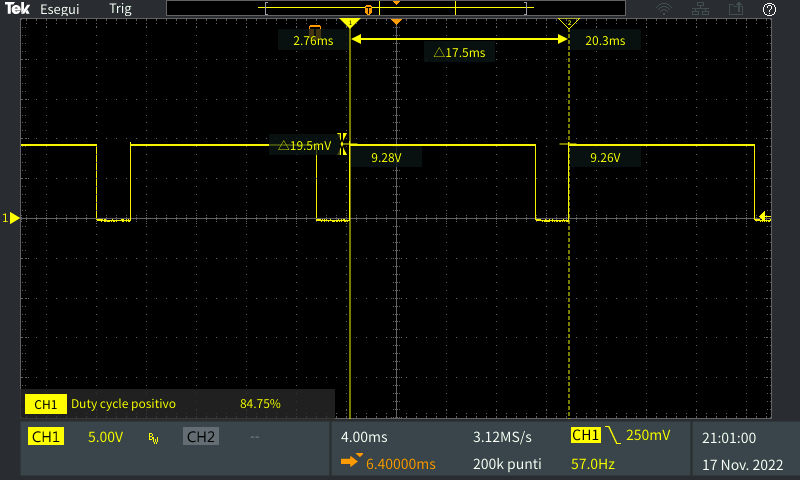
\includegraphics[width=\linewidth]{./ImageFiles/Laboratorio 5/TEK00014.PNG}
	\end{minipage}
	\begin{minipage}{.496\textwidth}
		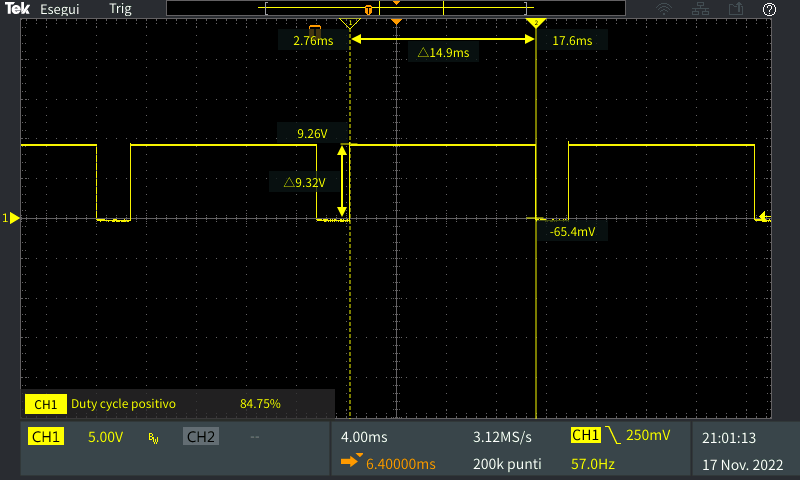
\includegraphics[width=\linewidth]{./ImageFiles/Laboratorio 5/TEK00015.PNG}
	\end{minipage}
	\caption{Segnale di uscita al circuito astabile realizzato con l'integrato LM555.}
	\label{fig:circuito_3_scope}
\end{figure}
Dalla equazione \ref{eq:3_1} si calcola che il valore teorico del duty-cycle con i valori indicati è pari a
\begin{equation}
	\delta=\frac{\SI{55.10}{\kilo\ohm}+\SI{12.00}{\kilo\ohm}}{\SI{55.10}{\kilo\ohm}+2\times\SI{12.00}{\kilo\ohm}}=\SI{84.83}{\percent},
\end{equation}
mentre il valore misurato tramite i cursori dell'oscilloscopio è pari a \SI{84.75}{\percent}, molto simile al valore teorico.

\noindent
Successivamente, si sono effettuate misure del duty-cycle e della frequenza del segnale ottenuto variando il valore delle resistenze $R_A$ ($R_B$ mantenuta constante con valore di \SI{12}{\kilo\ohm}) e della capacità $C$. I dati ottenuti sono stati riportati nella figura \ref{fig:circuito_3_plot}.\todo{immagini da rifare}
\begin{figure}[tbh]
	\centering
	\begin{minipage}{.496\textwidth}
		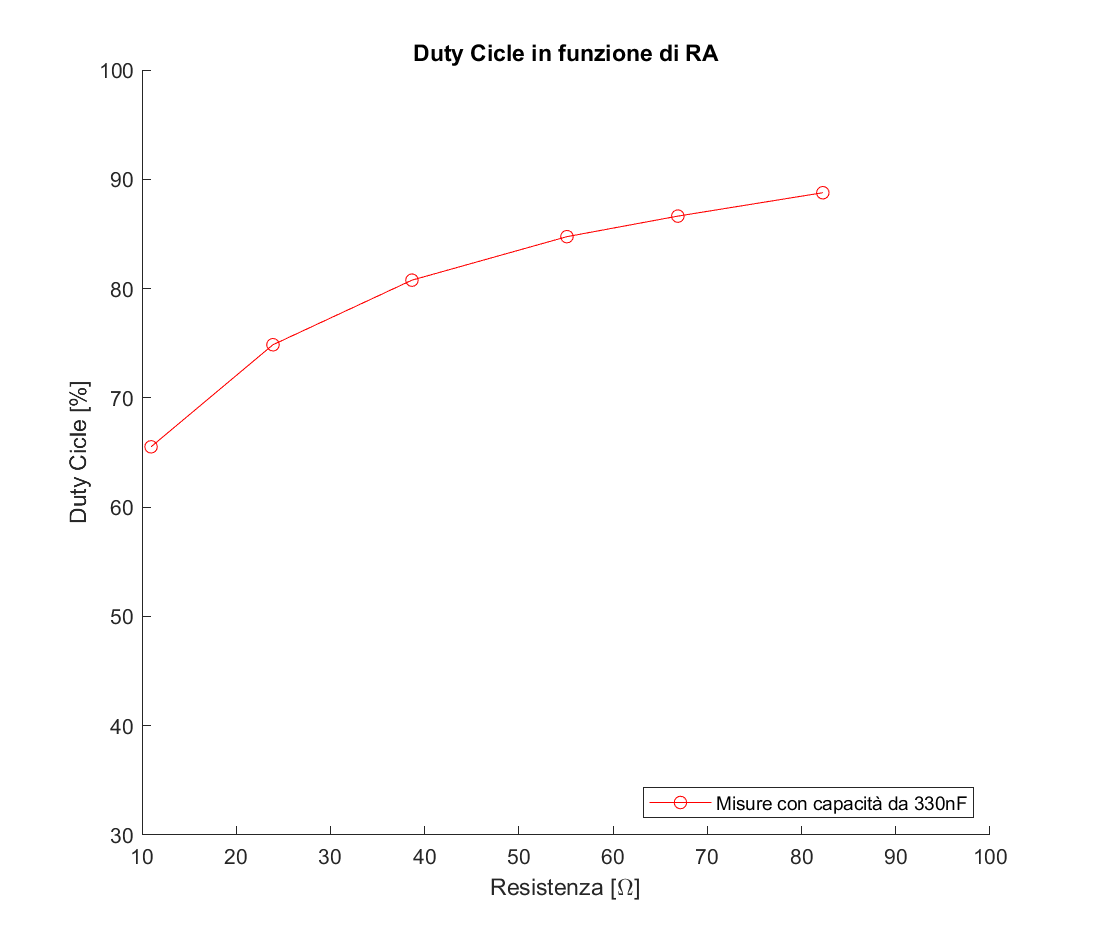
\includegraphics[width=\linewidth]{./ImageFiles/Laboratorio 5/Duty vs RA}
	\end{minipage}
	\begin{minipage}{.496\textwidth}
		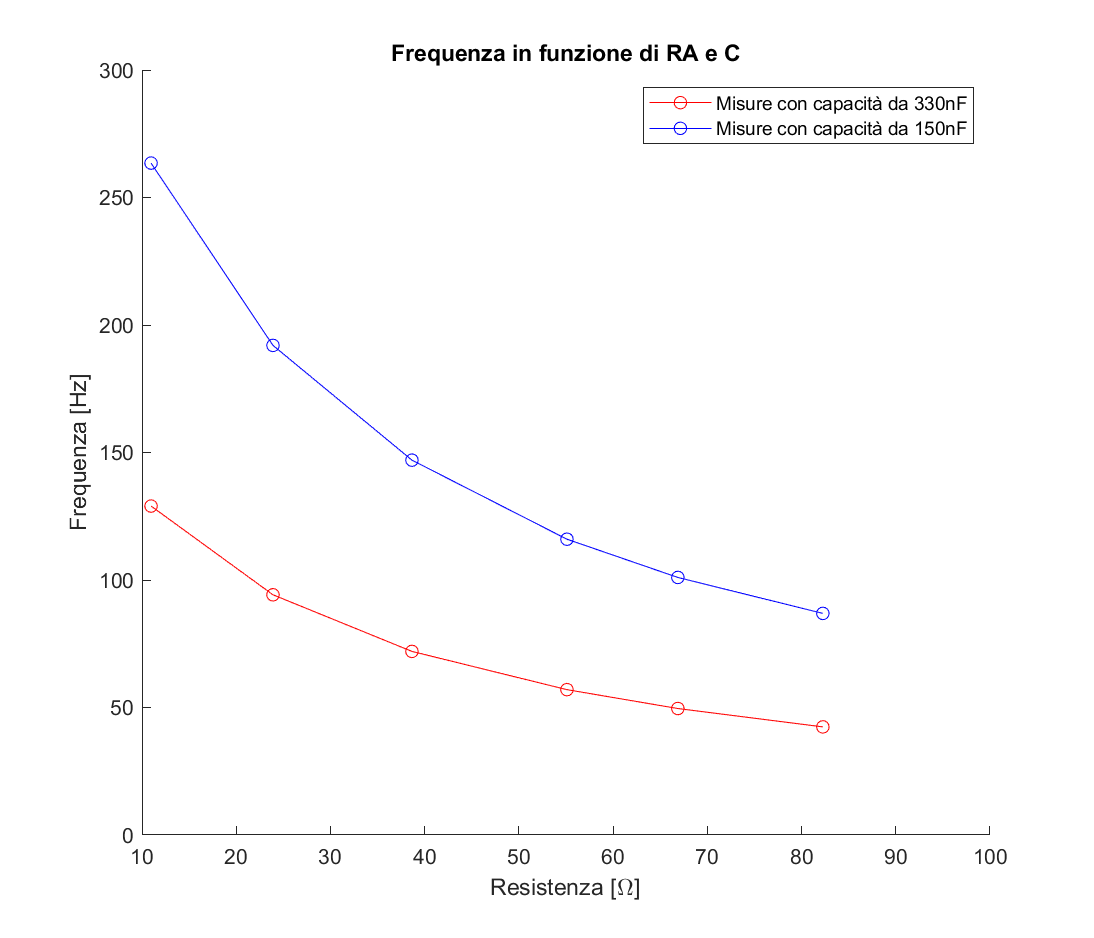
\includegraphics[width=\linewidth]{./ImageFiles/Laboratorio 5/F vs RA}
	\end{minipage}
	\caption{Misure del duty-cycle e della frequenza del segnale in uscita dal circuito in funzione della resistenza R\sub{A} e R\sub{B} e della capacità C.}
	\label{fig:circuito_3_plot}
\end{figure}


\clearpage
Il quarto circuito realizzato permette di superare i limiti sul valore minimo e massimo del duty-cycle presenti nel circuito precedente.

\begin{figure}[h!]
	\centering
	\begin{minipage}{.45\textwidth}
		\scalebox{.47}{
			\begin{circuitikz}
				%Main dip package
				\draw (0,0) node[dipchip,num pins=8, hide numbers, external pins width=0.1, scale=3, external pad fraction=6](C){LM555};
				%Pin names
				\node [right] at (C.bpin 1) {GND};
				\node [right] at (C.bpin 2) {Trigger};
				\node [right] at (C.bpin 3) {Output};
				\node [right] at (C.bpin 4) {Reset};
				\node [left] at (C.bpin 5) {Control Voltage};
				\node [left] at (C.bpin 6) {Threshold};
				\node [left] at (C.bpin 7) {Discharge};
				\node [left] at (C.bpin 8) {$V_{CC}$};
				%Connections
				\draw (C.pin 1) -- ++(-2.9,0) ++(-.1,0) node[jump crossing](crgnd){} ++(-.1,0) -- ++(-.9,0) -- ++(0,-6.5) node[ground]{};
				\draw (C.pin 8) -- ++(.9,0) ++(.1,0) coordinate(vccj) node[jump crossing]{} ++(.1,0)-- ++(.9,0) coordinate(vcc) -- ++(0,1.35) node[vcc]{$V_{CC}$};
				\draw (C.pin 7) -- ++(2,0) coordinate(dsc) to[R=$R_A$] (vcc);
				\draw (C.pin 5) -- ++(.9,0) ++(.1,0) node[jump crossing]{} ++(.1,0) -- ++(.9,0) to[C=$C_2$] ++(0,-1.5) node[ground]{};
				\draw (C.pin 6) -- ++(1,0) -- ++(0,-3.6) -- ++(-8.9,0) to[short, -*] ++(0,5.28);
				\draw (C.pin 4) -- ++(-1.5,0) -- ++(0,3) to[crossing] ++(0,.72) to[crossing] ++ (0,2.64) node[vcc]{$V_{CC}$};
				\draw (C.pin 3) to[short, -o] ++(-1,0) ++(0,.1) node[above]{$v_{out}$};
				\draw (C.pin 2) -- ++(-3,0) coordinate(vin);
				\draw (-1.5,4.02) coordinate (d1) to[potentiometer, name=P] ++(0,3) coordinate(d2);
				\coordinate (d1sh) at ([xshift=1mm, yshift=1mm]d1);
				\draw [to-, thick](d2)+(1mm,-1mm) to [out=-45,in=45] node[right, midway] {$R_{T}$} (d1sh);
				\draw [to-, thick](d1)+(-1mm,1mm) to [out=180-45,in=-90] node[left, midway] {$R_{T1}$} (P.wiper);
				\draw [to-, thick](d2)+(-1mm,-1mm) to [out=180+45,in=90] node[left, midway] {$R_{T2}$} (P.wiper);
				\draw (d1) to[D=$D_1$, invert] ++(3,0) -- ++(0,1.5) coordinate(dend);
				\draw (d2) to[D=$D_2$] ++(3,0) -- (dend);
				\draw (vin) -- (crgnd) -- ++(0,3) coordinate(tb) to[short, -*] (P.wiper);
				\draw (dend) to[short, *-] (tb-|vccj) -- (vccj) to[short, -*] (C.pin 7 -| vccj);
				\draw (vin) to[C=$C$] ++(0,-4.82) node[ground]{};
				\draw[thick] (-8,-5.3) rectangle (6.6,8.2);
			\end{circuitikz}
		}
	\end{minipage}\qquad
	\begin{minipage}{.45\textwidth}
		\includegraphics[width=\linewidth]{./ImageFiles/Laboratorio 5/CIR4.jpg}
	\end{minipage}
	\caption{Schema circuitale e foto del circuito realizzato.}
	\label{fig:circuito_4}
\end{figure}

\noindent
Per ottenere un duty-cycle selezionabile nell'intervallo dallo \SI{0}{\percent} al \SI{100}{\percent}, si introducono i diodi $D1$ e $D2$ e il trimmer $T$ (\Fig\ref{fig:trimmer}).
\begin{figure}[tbh]
	\centering
	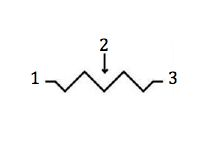
\includegraphics[width=0.2\linewidth]{./ImageFiles/Laboratorio 5/trimmer.jpg}
	\caption{Simbolo circuitale di un trimmer.}
	\label{fig:trimmer}
\end{figure}
Il trimmer viene utilizzato come resistenza variabile e permette di variare il valore della resistenza attraverso la quale la capacità $C$ si carica e scarica. Infatti, la corrente che carica il condensatore fluisce attraverso la resistenza $R_A$, il diodo e la resistenza $R_{T_1}$, ossia la resistenza tra il terminale 3 e 2 del trimmer. Al contrario, la capacità di scarica solo attraverso la resistenza $R_{T_2}$, ossia la resistenza tra il terminale 1 e 2 del trimmer. Le equazioni che descrivono il tempo di carica e scarica delle capacità diventano quindi:
\begin{equation}
	\begin{split}
		T_1(\text{carica})&=\ln{2}\ C\left(R_A+R_{T_1}\right), \\
		T_2(\text{scarica})&=\ln{2}\ C\left(R_{T_2}\right).
	\end{split}
\end{equation}
Indicando con $R_T$ la resistenza tra il terminale 1 e 3 del trimmer (che equivale alla somma delle resistenze $R_{T_1}$ e $R_{T_2}$) otteniamo:
\begin{equation}
	\begin{split}
		T_2&=\ln{2}\ C\left(R_T-R_{T_1}\right) \\
		T&=T_1+T_2=\ln{2} C\left(R_A+\cancel{R_{T_1}}+R_T-\cancel{R_{T_1}}\right) \\
		T&=\ln{2}\ C\left(R_A+R_T\right) \\
		\frac{T_1}{T}&=\frac{\ln{2}\ C\left(R_A+R_{T_1}\right)}{\ln{2}\ C\left(R_A+R_T\right)} \\
		\delta&=\frac{R_A+R_{T_1}}{R_A+R_T}
	\end{split}
\end{equation}